\newcommand{\package}{\emph}

\setcounter{chapter}{1}
\setcounter{section}{0}
\section{Chromosomal instability}
\subsection{a}
Calculate three ratios $C= \frac{CIN}{no-CIN}$ and show that $C$ is independent of time
1.	Neutral CIN : if we assume that genes with CIN are neutral (have no fitness advantages or disadvantages) we can conclude that mutation rate from state $A(+-) \rightarrow A(--)$ is $Nu_2$ and from $A (+- CIN) \rightarrow A(-- CIN)$ is $Nu_3$. So we can create a linear ODE system. 
From lecture we know that its solutions for  $X_2$ (i.e. A(--)) and $Y_2$ (i.e. A(-- CIN)) are the following:
\[X_2(t) \approx Nu_1u_2 \times \frac{t^2}{2} \]
\[Y_2(t) \approx u_1u_ct^2\]
So, our rate is

\[ \frac{Y_2}{X_2} = \frac{u_1u_ct^2}{\frac{Nu_1u_2t^2}{2}} = \frac{2u_c}{Nu_2}\]

We can see that there is no time variable here, so the process is independent of time. 
Now remembering that $U_c = 2\times n_1\times(u+p_0)+2\times n_2\times u$  and  $U_2 = u+p_0$ and substituting it into equation above we have

\[ C_1 = \frac{2u_c}{Nu_c} = \frac{4n_1(u+p_0) + 4n_2u}{N(u+p_0)} = \frac{4n_1(2u)+4n_2u}{N(2u)} = \frac{4n_1+2n_2}{N}\]

2. Costly CIN in small compartments: if we assume that genes with CIN have fitness less then 1 ($r<1$) (probably because of defense system like apoptosis etc) we shall modify the ODE system above , because $U_c$ (mutation of normal allele into CIN allele) now is not just $U_c$ but depends on fitness $R_c$ and population size $N$, so can be calculated by Moran Process. So, no $U_c = N\times p \times U_c$  now.
Now, the solution of that new ODE system is:

\[ X_2 \approx \frac{Nu_1u_2t^2}{2} ; Y_2 \approx Npu_1u_ct^2 \]

So, our final ratio is

\[ C_2 = \frac{Y_2}{X_2} = \frac{2pu_c}{u_2} = \frac{4n_1p(u+p_0) + 4n_2up}{u+p_0} = \frac{4n_1p(2u)+4n_2up}{2u} = 4n_1p+2n_2p \]

where $p$ is determined by Moran Process as follows:

\[  p = \frac{1-\frac{1}{r}}{1-\frac{1}{r^N}} \]

We can see C2 is also independent of time.

3.	Costly CIN in large compartments: for large compartments we will never achive Y0 and Y1 states (A(++)CIN  and A(+-CIN) )  because $N p U_c$ is vanishingly small, but new tunnel transition from $X_1$ to $Y_2$ CIN will play its role. That new rate $R$ can be calculated as follows:

\[ R = \frac{Nu_cru_3}{1-r} \]

So, new ODE system has the following solutions:

\[ X_2 \approx \frac{Nu_1u_2t^2}{2} ; Y_2 \approx \frac{Ru_1t^2}{2} \]

So our rate is

\[ C_3 = \frac{Y_2}{X_2} = \frac{R}{Nu_2} = \frac{u_cru_3}{(1-r)u_2} = \frac{(2n_1(2u)+2n_2u)ru_3}{(1-r)2u} = \frac{(2n_1+n_2)ru_3}{1-r}\]

\subsection{b}
Computing the real values of c:

1. Neutral CIN

\[ C = \frac{4n_1+2n_2}{N} = \frac{4\times 5+2 \times 3}{10} = \boxed{2.6} \]

2. Costly CIN in small compartments

\[ p = \frac{1-\frac{1}{r}}{1 - \frac{1}{r^N}} = \frac{1-\frac{1}{0.9}}{1-\frac{1}{0.9^{10}}} = 0.05948  \]
\[ C_2 = 4n_1p+2n_2p = 2p(2n_1+n_2 )=2\times0.05948(2\times5+3)=\boxed{1.5465} \]

3. Costly CIN in large compartments

\[ C_3=\frac{((2n_1+n_2)ru_3)}{(1-r)}=\frac{((2\times5+3)0.9\times0.01)}{(1-0.9)}=\boxed{1.17} \]


\setcounter{chapter}{2}
\setcounter{section}{0}
\section{Linear process of colonic crypt transformation}

\textbf{1. Homogenous tissue} (well-mixed compartment).\\
First, we will find a prob of a single mutant with fitness $r=1.05$ to take over the compartment of size $N=1000$ (Moran Process)

\[ p = \frac{1-\frac{1}{r}}{1 - \frac{1}{r^N}} = \frac{1-\frac{1}{1.05}}{1-\frac{1}{1.05^{1000}}} = 0.0476  \]

Then, we find the prob of a compartment has been taken by mutated cell after 50 years (25550 days) is 

\[ p=1-e^{-Nupt}=1-e^{-1000\times10^{-8}\times0.0476\times18250}=0.0086528 \]

Now, we have $M=10^7$ crypts so we could expect $M \times 0.0086528 =$  \textbf{86528 neoplastic crypts}

\textbf{2. Single Stem cell} (linear process). \\

Since the stem cell is the only one which is mater in linear crypt, we could calculate the probability of compartment being taken by mutation of a stem cell in 50 years as follows $t = 50\times\frac{365}{10}=1825 $:

\[ p=1-e^{-ut}=1-e^{-10^{-8}\times1825}=1.825\times10^{-5} \]

so, we expect $10^7 \times p =$  \textbf{182.5 neoplastic crypts}

\textbf{3.	Multiple stem cells} (5 cells)\\

 This is actually the same case as well-mixed compartment but with effective population size of 5, because any of stem cell can mutate and originate a cancer, so 

\[ p = \frac{1-\frac{1}{r}}{1 - \frac{1}{r^N}} = \frac{1-\frac{1}{1.05}}{1-\frac{1}{1.05^{5}}} = 0.22  \]
\[ p=1-e^{-Nupt}=1-e^{-5\times10^{-8}\times0.22\times18250}=2.0075\times10^{-5} \]

so, we expect $10^7 \times p = $ \textbf{200.74 neoplastic crypts}
\setcounter{chapter}{3}
\setcounter{section}{0}
\section{Multistage Theory}
\begin{figure}[htbp]
\centering
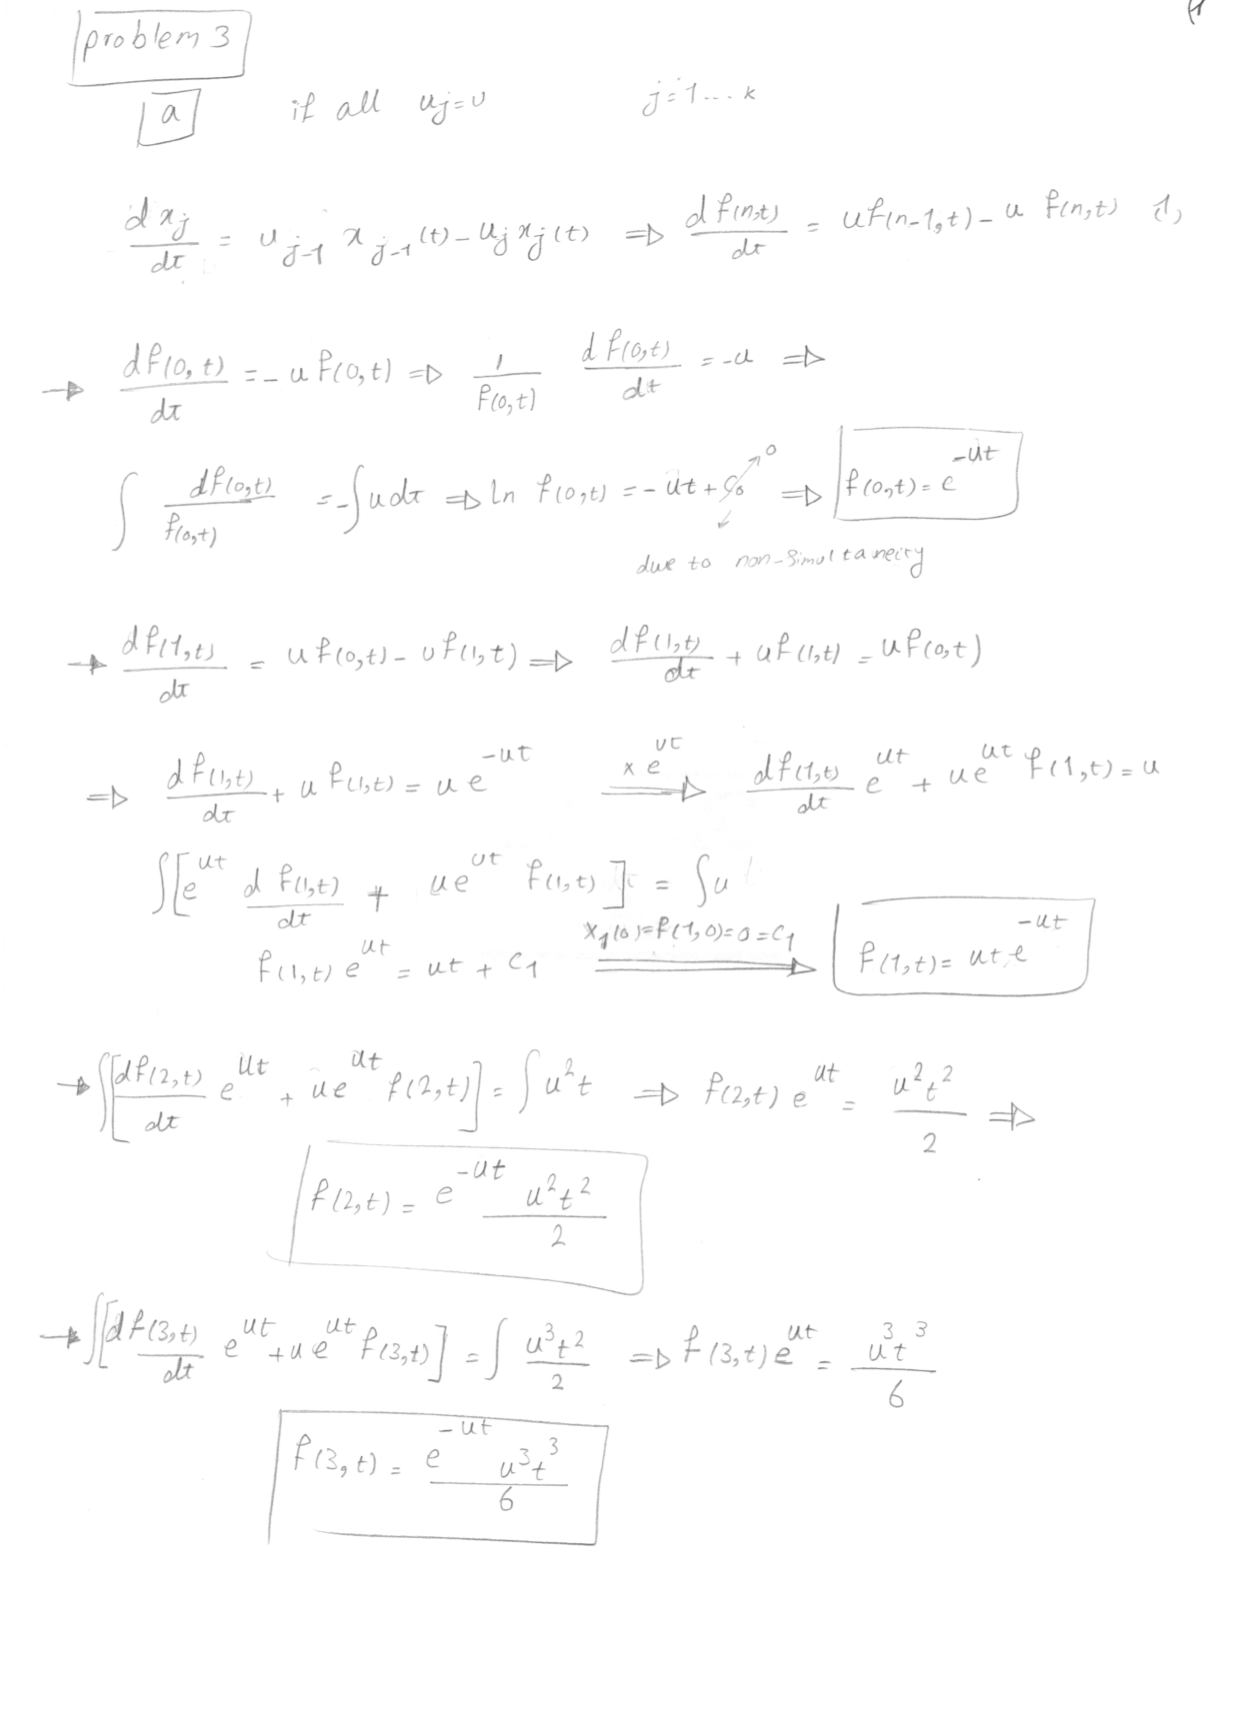
\includegraphics[scale=0.8, page=1]{./img/ex3}
\end{figure}
\begin{figure}[htbp]
\centering
\includegraphics[scale=0.8, page=2]{./img/ex3}
\end{figure}
\newpage
\setcounter{chapter}{4}
\setcounter{section}{0}
\section{Pathways of carcinogenesis}
\subsection{a}
The probability of the path $ P = 2 \rightarrow 3 \rightarrow 1 $ for three independent mutations occurring after exponentially distributed waiting time $T_i \sim exp(\lambda_i), i = 1,2,3$ is:

\[ P = J_1 \rightarrow \dots \rightarrow J_k = J_2 \rightarrow J_3 \rightarrow J_1  \]
\begin{center}
\begin{tikzpicture}[
back line/.style={densely dotted},
hligh line/.style={preaction={draw=yellow,-,double=yellow,double distance=6\pgflinewidth}},
cross line/.style={preaction={draw=white, -,line width=6pt}}]
\matrix (m) [matrix of math nodes,
row sep=2em, column sep=2em,
text height=1.5ex,
text depth=0.25ex]{
& \{2,3\} & & \{1,2,3\}\\
\{3\}& & \{3,1\}\\
& \{2\} & & \{1,2\}\\
\{0\} & & \{1\} \\
};
\path[->]
(m-1-2) edge [hligh line] (m-1-4) 
(m-2-1) edge (m-1-2) 
(m-2-1) edge [cross line] (m-2-3) 
(m-2-3) edge (m-1-4) 
(m-3-2) edge [hligh line] (m-1-2) edge [back line] (m-3-4)
(m-3-4) edge (m-1-4)
(m-4-1) edge (m-4-3) edge (m-2-1) edge [hligh line] (m-3-2)
(m-4-3) edge [cross line] (m-2-3) edge (m-3-4);
\end{tikzpicture}
\end{center}

\[ \text{Prob(P)} = \prod\limits_{i=1}^{3} \frac{\lambda_{Ji}}{\sum\limits_{J \in \text{Exit}_i} \lambda_J } = \frac{\lambda_2}{\sum\limits_{J \in \text{Exit}_i = 1,2,3} \lambda_J} \times \frac{\lambda_3}{\sum\limits_{J \in \text{Exit}_i = 1,3} \lambda_J}  \times \frac{\lambda_1}{\sum\limits_{J \in \text{Exit}_i = 1} \lambda_J} =\boxed{ \frac{\lambda_2\lambda_3}{(\lambda_1+\lambda_2+\lambda_3)\times(\lambda_3+\lambda_1)}}\]

\subsection{b}

All possible genotypes starting from the wt (no mutation occurred) are 8: $\{0\};\{1,2,3\};\{12,23,31\};\{123\}$. Considering 2 out of 3 mutations one will obtain 6 possible pathways.
Then, the expected waiting time is (where $k$ is the number of mutations expected and $p$ the number of pathways):

\[E[T_k] = \sum\limits_{p=1}^{6} \sum\limits_{n=1}^{k=2} \frac{1}{\sum\limits_{J \in \text{Exit}_i} \lambda_J} \times \text{Prob}(P) = \sum\limits_{p=1}^{6} \sum\limits_{n=1}^{k=2} \frac{1}{\sum\limits_{J \in \text{Exit}_i} \lambda_J} \times \prod\limits_{i=1}^{3} \frac{\lambda_{Ji}}{\sum\limits_{J \in \text{Exit}_i} \lambda_J } \]

\fbox{
 \addtolength{\linewidth}{-1\fboxsep}%
 \addtolength{\linewidth}{-1\fboxrule}%
 \begin{minipage}{\linewidth}
\begin{align*}
E[T_{p_{1-6}}] = & (\frac{1}{\lambda_1+\lambda_2+\lambda_3} + \frac{1}{\lambda_2+\lambda_3}) \times (\frac{\lambda_1}{\lambda_1+\lambda_2+\lambda_3}) + \\ 
+ &(\frac{1}{\lambda_1+\lambda_2+\lambda_3} + \frac{1}{\lambda_1+\lambda_3}) \times (\frac{\lambda_2}{\lambda_1+\lambda_2+\lambda_3}) + \\ 
+ &(\frac{1}{\lambda_1+\lambda_2+\lambda_3} + \frac{1}{\lambda_1+\lambda_2}) \times (\frac{\lambda_3}{\lambda_1+\lambda_2+\lambda_3}) 
\end{align*}
\end{minipage}
}
\subsection{c}

Considering $d$ independent mutation, there are exactly $d\times(d-1)\times(d-2)\times\dots\times1 = d!$ pathways to the genotype where all the mutations are present at the same time. If cancer arises after $k$ mutation, there are $d\times(d-1)\times(d-2)\times\dots\times(d-k+1) = \frac{d!}{(d-k)!}$ paths.

\setcounter{chapter}{5}
\setcounter{section}{0}
\section{Neutral Wright-Fisher process}
\begin{figure}[htbp]
\centering
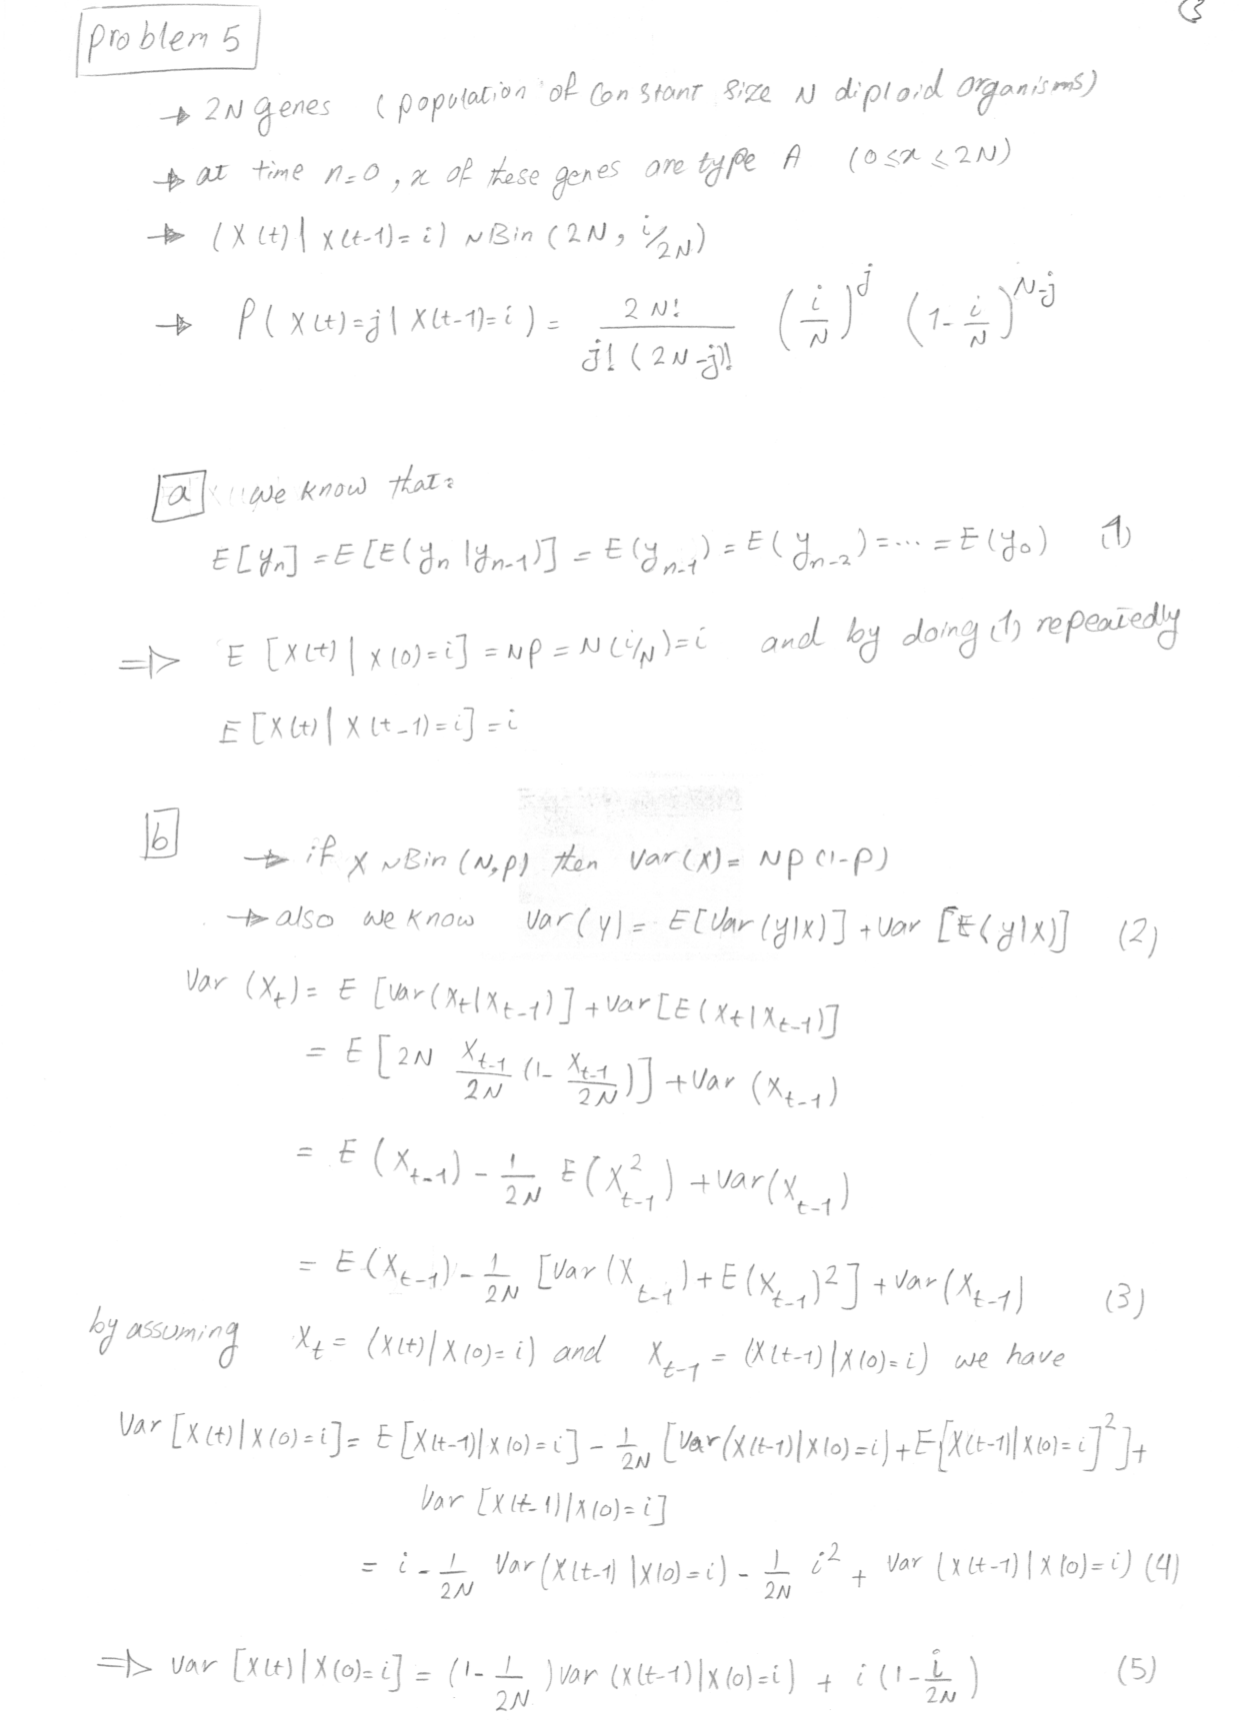
\includegraphics[scale=0.8, page=1]{./img/ex5}
\end{figure}
\begin{figure}[htbp]
\centering
\includegraphics[scale=0.8, page=2]{./img/ex5}
\end{figure}
\newpage


\setcounter{chapter}{6}
\setcounter{section}{0}
\section{Wave approximation}
\[ x'_j = sx_j (j-<j>)  \]
\[ s<j> = s\sum\limits_{j}jx_j = \text{constant} \]

\subsection{a}

\begin{align*}
 x'_j = sx_j(j-<j>)	\Rightarrow & \frac{dx_j(t)}{x_j(t)} = s(j-<j>)dt\\
& \int\limits_{x(0)}^{x(t)} \frac{dx_j(t)}{x_j(t)} = \int\limits_{0}^{t} s(j-<j>)dt\\
& \ln x_j(t) - \ln x_j(0) = st(j-<j>) -s0(j-<j>) = st(j-<j>)\\
& e^{\ln x_j(t)- \ln x_j(0)} = e^{st(j-<j>)}\\
& \frac{x_j(t)}{x_j(0)} = e^{st(j-<j>)}
\end{align*}

As $x_j(0) = \frac{1}{N} \Rightarrow \boxed{x_j(t) = \frac{e^{st(j-<j>)}}{N}} $

\subsection{b}

$r = udx_j(t)$, let $T$ be the time it takes to produce a new mutant $x_{j+1}(T) = \frac{1}{N} = ud\int\limits_{0}^{T} x_j(t)dt$.\\
Replacing $x_j(t) = \frac{e^{j-<j>}}{N} : $
\begin{align*}
\frac{1}{N} = ud\int\limits_{0}^{T} \frac{1}{N}e^{(j-<j>)}dt &= \frac{ud}{N}\int\limits_{0}^{T} e^{st(j-<j>)}dt\\
1 = ud\left(\frac{e^{sT(j-<j>)}}{s(j-<j>)}-\frac{e^{s0(j-<j>)}}{s(j-<j>}\right) &= ud\left( \frac{e^{sT(j-<j>)}}{s(j-<j>)} - \frac{1}{s(j-<j>)}\right)\\
 \frac{1}{ud}+\frac{1}{s(j-<j>)} &= \frac{e^{sT(j-<j>)}}{s(j-<j>)}\\
 \frac{s(j-<j>)}{ud}+1 &= e^{sT(s(j-<j>))}\\
 \ln (\frac{s(j-<j>)}{ud}+1) &= sTs(j-<j>\\
 \Aboxed{T &= \frac{\ln(1+\frac{s(j-<j>))}{ud})}{s(j-<j>)}}
\end{align*}

\subsection{c}

For $u=10^{-7}$, $d=100$, $s=0.01$ per mutation, $(j-<j>) \approx \sqrt{\log N}$, $N=10^{7}$ cells, generation time $t=1$ day.
From point b: $\boxed{T = \frac{\ln(1+\frac{s(j-<j>))}{ud})}{s(j-<j>)}}$.

\begin{align*}
T &= \frac{\ln(1+\frac{s(j-<j>))}{ud})}{s(j-<j>)} =& \frac{\ln (1+\frac{s\sqrt{\ln H}}{nd})}{s\sqrt{\ln N}} \\
T &= \frac{\ln (1+\frac{0.01\sqrt{\ln 10^7}}{10^{-7}\times 100})}{0.01\sqrt{\ln 10^7}} \rightarrow & T \approx 207 \text{days}
\end{align*}


